% System Integration and Testing: Inventory Management System (StockPilot)
% Compile with: pdflatex system-testing.tex   (run twice for the table of contents)
\documentclass[11pt,a4paper]{article}
\usepackage[T1]{fontenc}
\usepackage{lmodern}
\usepackage[margin=2.5cm]{geometry}
\usepackage{booktabs}
\usepackage{tabularx}
\usepackage{longtable}
\usepackage{array}
\newcolumntype{Y}{>{\raggedright\arraybackslash}X}
\newcolumntype{P}[1]{>{\raggedright\arraybackslash}p{#1}}
\usepackage{enumitem}
\usepackage{fancyhdr}
\usepackage{xcolor}
\usepackage{amssymb}
\usepackage{upquote}
\usepackage{listings}
\usepackage{graphicx}
\usepackage{float}
\usepackage{needspace}
\usepackage[hidelinks]{hyperref}
\hypersetup{colorlinks=true, linkcolor=blue, urlcolor=blue}

\pagestyle{fancy}
\fancyhf{}
\fancyhead[L]{Inventory Management System}
\fancyhead[R]{System Integration and Testing}
\fancyfoot[C]{\thepage}
\renewcommand{\headrulewidth}{0.4pt}
\setlength{\headheight}{14pt}
\setlength{\parskip}{0.35em}
\setlength{\parindent}{0pt}
\setlist{itemsep=0.15em, topsep=0.3em}

\newcommand{\code}[1]{\texttt{#1}}

\definecolor{querybg}{HTML}{F1F4F8}
\definecolor{rule}{HTML}{B8C0CC}
\lstdefinestyle{query}{
  basicstyle=\ttfamily\small, backgroundcolor=\color{querybg}, columns=fullflexible,
  keepspaces=true, breaklines=true, showstringspaces=false, frame=single, rulecolor=\color{querybg},
  framesep=5pt, xleftmargin=6pt, xrightmargin=6pt, aboveskip=0.6em, belowskip=0.6em
}
\lstdefinestyle{result}{
  basicstyle=\ttfamily\footnotesize, columns=fullflexible, keepspaces=true, breaklines=true,
  showstringspaces=false, frame=leftline, framerule=1.5pt, rulecolor=\color{rule},
  framesep=8pt, xleftmargin=12pt, aboveskip=0.3em, belowskip=0.8em
}

\begin{document}

\begin{titlepage}
  \centering
  \vspace*{3cm}
  {\LARGE\bfseries Inventory Management System\par}
  \vspace{0.4cm}
  {\Large Using MERN Stack\par}
  \vspace{1.5cm}
  {\Large\bfseries Step 5: System Integration and Testing\par}
  \vspace{0.4cm}
  {\large Integration of the Three Parts,\\ Test Plan, Test Cases and Results\par}
  \vfill
  {\large Web Engineering Lab Project\par}
  \vspace{0.3cm}
  {\large Jashore University of Science and Technology\par}
  \vspace{2cm}
\end{titlepage}

\tableofcontents
\newpage

\section{Introduction}
This document covers the fifth step of the project, \textbf{System Integration and Testing}. The earlier steps built and tested the parts one by one: the database (Step 2), the backend (Step 3) and the frontend (Step 4). In this step the three parts are joined into one system, and the whole system is tested the way a user works with it.

Amounts of money are written as Tk in this document. The website shows the taka sign.

\section{System Integration}
\subsection{The three parts and their connections}
\begin{table}[h]
\centering
\begin{tabularx}{\textwidth}{@{}P{3.2cm}P{3.6cm}Y@{}}
\toprule
\textbf{Connection} & \textbf{How} & \textbf{Setting} \\
\midrule
Frontend to backend & HTTP requests with JSON and a JWT token & \code{NEXT\_PUBLIC\_API\_BASE\_URL} in the frontend; \code{CLIENT\_URL} (CORS) in the backend \\
Backend to database & Mongoose connection & \code{MONGO\_URI} in the backend \\
\bottomrule
\end{tabularx}
\caption{Connections between the parts}
\end{table}

The integration was done from the bottom up. First the backend was connected to the database and tested through its API. Then the frontend was connected to the backend. Because of this order, a problem found in this step can only be in the newest connection.

\subsection{Environments}
The same code runs in three environments. Only the settings are different.
\begin{table}[h]
\centering
\begin{tabularx}{\textwidth}{@{}P{2.3cm}P{2.9cm}P{2.9cm}Y@{}}
\toprule
\textbf{Environment} & \textbf{Frontend} & \textbf{Backend} & \textbf{Database} \\
\midrule
Development & \code{localhost:3000} & \code{localhost:5000} & \code{inventory\_management\_system} \\
Test & \code{localhost:3000} & \code{localhost:5050} & \code{stockpilot\_api\_test} \\
Production & Vercel & Render & \code{inventory\_management\_system} \\
\bottomrule
\end{tabularx}
\caption{The three environments}
\end{table}
All tests that create or change data use the test environment, so the real data is never changed by a test.

\section{Test Plan}
The system is tested on five levels. Each level joins more parts than the level before.
\begin{table}[h]
\centering
\begin{tabularx}{\textwidth}{@{}P{2.4cm}P{2.6cm}YP{2.6cm}@{}}
\toprule
\textbf{Level} & \textbf{Tool} & \textbf{What is tested} & \textbf{Result} \\
\midrule
Unit tests & Vitest & Small parts of the backend alone, without a database: token check, role check, login limit, input validation & 19 of 19 passed \\
Integration tests & Vitest + MongoDB & Backend and a real database together: the money features, also with two requests at the same moment & 8 of 8 passed \\
API tests & Postman & Every route of the backend through HTTP: 92 requests, 217 checks & 217 of 217 passed \\
System tests & By hand, in the browser & Frontend, backend and database together, as a user works: 27 cases & 21 passed, 6 not run \\
Deployment tests & By hand, live website & The three parts on three servers: 3 cases & Not run \\
\bottomrule
\end{tabularx}
\caption{Test levels and results}
\end{table}

\section{Automatic Tests}
\subsection{Unit and integration tests}
\begin{lstlisting}[style=query]
cd server
pnpm test               # unit tests
pnpm test:integration   # integration tests on a real MongoDB database
\end{lstlisting}
The unit tests need no database and finish in a few seconds. The integration tests start the real backend code against a separate MongoDB database. They cover the three money features: a walk-in sale is paid in full, a customer return can be cancelled, and supplier payments are tracked without overpaying. Two of these tests send two requests at the same moment and confirm that only one succeeds. This shows that the system stays correct when two users work at the same time.

\subsection{API tests}
The Postman collection of Step 3 calls all 55 routes of the backend with 92 requests. All 217 checks passed. The details are in the Step 3 document.

\section{System Tests}
\subsection{Preparation}
The system tests use the website in the browser, connected to the test backend and the test database.
\begin{lstlisting}[style=query]
# Terminal 1: backend on the test database (port 5050)
cd server
pnpm dev:apitest --reset

# Terminal 2: frontend that talks to the test backend (port 3000)
$env:NEXT_PUBLIC_API_BASE_URL = "http://localhost:5050/api/v1"
pnpm dev
\end{lstlisting}
The option \code{--reset} empties the test database, so every test run starts from the same state. The website is opened at \code{http://localhost:3000}. The test logins are \code{admin@stockpilot.test} / \code{AdminPass123} and \code{staff@stockpilot.test} / \code{StaffPass123}.

The cases are run in order, because each case uses the data of the cases before it. One product is followed through its whole life: it is bought, sold, damaged and returned. After every step the stock and the amounts of money are checked.

\needspace{10\baselineskip}
\subsection{Login and master data}
\begin{longtable}{@{}P{0.75cm}P{6.0cm}P{5.3cm}P{1.3cm}@{}}
\toprule
\textbf{ID} & \textbf{Steps} & \textbf{Expected result} & \textbf{Result} \\
\midrule
\endhead
S01 & \textbf{Login with a wrong password.} Open the website. Enter \code{admin@stockpilot.test} and the password \code{wrong123}. Press Sign in. & A red error message appears. The login page stays open. & Not run \\\addlinespace
S02 & \textbf{Login as Administrator.} Enter \code{admin@stockpilot.test} and \code{AdminPass123}. Press Sign in. & The Dashboard opens. Total products is 0. & Pass \\\addlinespace
S03 & \textbf{Create a category and a brand.} Categories: add \code{Smartphone}. Brands: add \code{Samsung}. & Both appear in their lists as Active. & Pass \\\addlinespace
S04 & \textbf{Create a product.} Products, New product: name \code{Galaxy A15}, SKU \code{GA15}, category Smartphone, brand Samsung, purchase price 18000, selling price 21000, minimum stock 5. Save. & The product is in the list with stock 0 and price Tk~21,000. & Pass \\\addlinespace
S05 & \textbf{Create a product with the same SKU.} New product again with any name and the SKU \code{GA15}. Save. & An error message says that the SKU already exists. No second product is created. & Pass \\\addlinespace
S06 & \textbf{Create a supplier and a customer.} Suppliers: add \code{Tech Supply}. Customers: add \code{Rahim Traders}. & Both appear in their lists. & Pass \\*
\bottomrule
\end{longtable}

\needspace{10\baselineskip}
\subsection{Purchase}
\begin{longtable}{@{}P{0.75cm}P{6.0cm}P{5.3cm}P{1.3cm}@{}}
\toprule
\textbf{ID} & \textbf{Steps} & \textbf{Expected result} & \textbf{Result} \\
\midrule
\endhead
S07 & \textbf{Create a purchase draft.} Purchases, New purchase: supplier Tech Supply, product Galaxy A15, quantity 10, unit price 18000. Create draft. & A draft purchase with total Tk~180,000 is in the list. Inventory still shows stock 0. & Pass \\\addlinespace
S08 & \textbf{Complete the purchase.} Press Complete on the draft. & The status is Completed and Outstanding is Tk~180,000. Inventory shows stock 10. & Pass \\\addlinespace
S09 & \textbf{Pay the supplier.} Press Pay supplier. Amount 100000, method Bank transfer. Save. & Outstanding becomes Tk~80,000. & Pass \\\addlinespace
S10 & \textbf{Pay more than is owed.} Press Pay supplier again. Amount 90000. Save. & An error message appears. Outstanding stays Tk~80,000. & Pass \\*
\bottomrule
\end{longtable}

\needspace{10\baselineskip}
\subsection{Sale and payment}
\begin{longtable}{@{}P{0.75cm}P{6.0cm}P{5.3cm}P{1.3cm}@{}}
\toprule
\textbf{ID} & \textbf{Steps} & \textbf{Expected result} & \textbf{Result} \\
\midrule
\endhead
S11 & \textbf{Create a sale draft.} Sales, New sale: customer Rahim Traders, product Galaxy A15, quantity 2. Create draft. & A draft sale with total Tk~42,000 is in the list. Inventory still shows stock 10. & Pass \\\addlinespace
S12 & \textbf{Complete the sale.} Press Complete on the draft. & Status Completed, Unpaid, Outstanding Tk~42,000. Inventory shows stock 8. & Pass \\\addlinespace
S13 & \textbf{Collect a part payment.} Press Collect payment. Amount 20000, method Cash. Save. & The sale shows Partly paid and Outstanding Tk~22,000. & Pass \\\addlinespace
S14 & \textbf{Sell more than the stock.} New sale: customer Rahim Traders, Galaxy A15, quantity 50. Create draft. Then press Complete. & The message \code{Not enough stock for Galaxy A15} appears. The sale stays a draft and the stock stays 8. & Pass \\\addlinespace
S15 & \textbf{Cancel the draft.} Press Cancel on that draft. & The status is Cancelled. & Pass \\\addlinespace
S16 & \textbf{Walk-in sale.} New sale: leave the customer as Walk-in customer, method Cash, Galaxy A15, quantity 1. Create draft, then Complete. & The sale is Completed and Paid, Outstanding Tk~0. Inventory shows stock 7. & Pass \\*
\bottomrule
\end{longtable}

\needspace{10\baselineskip}
\subsection{Stock adjustment and returns}
\begin{longtable}{@{}P{0.75cm}P{6.0cm}P{5.3cm}P{1.3cm}@{}}
\toprule
\textbf{ID} & \textbf{Steps} & \textbf{Expected result} & \textbf{Result} \\
\midrule
\endhead
S17 & \textbf{Record a damaged unit.} Inventory, Adjust stock: Galaxy A15, type Damaged, quantity 1, any reason. Save. Then press History. & Stock is 6. The history lists the purchase, the two sales and the adjustment. & Pass \\\addlinespace
S18 & \textbf{Customer return.} Returns, Customer return: choose the sale of Rahim Traders, quantity 1, reason \code{Wrong colour}. Save. & The return is in the list. Inventory shows stock 7. The sale shows Outstanding Tk~1,000. & Pass \\\addlinespace
S19 & \textbf{Cancel the return.} Press Cancel on the return and give a reason. & The return shows Cancelled. Stock is 6 again and the sale shows Outstanding Tk~22,000 again. & Pass \\*
\bottomrule
\end{longtable}

\needspace{10\baselineskip}
\subsection{Totals on the report pages}
\begin{longtable}{@{}P{0.75cm}P{6.0cm}P{5.3cm}P{1.3cm}@{}}
\toprule
\textbf{ID} & \textbf{Steps} & \textbf{Expected result} & \textbf{Result} \\
\midrule
\endhead
S20 & \textbf{Dashboard.} Open the Dashboard and press Refresh. & Total products 1. Today's sales Tk~63,000 (2 completed sales). Total outstanding Tk~22,000. & Pass \\\addlinespace
S21 & \textbf{Payments and Dues.} Open Payments \& Dues. & Total paid Tk~41,000. Outstanding balance Tk~22,000. Owed to suppliers Tk~80,000. & Pass \\\addlinespace
S22 & \textbf{Reports.} Open Reports and choose This month. & Total sales Tk~63,000. Total purchases Tk~180,000. Gross profit Tk~9,000. Current stock value Tk~108,000. & Pass \\\addlinespace
S23 & \textbf{Audit log.} Open Audit Log. & The actions of this test (create, complete, payment, return, cancel) are listed with the user and the time. & Not run \\*
\bottomrule
\end{longtable}

\needspace{10\baselineskip}
\subsection{Roles, session and failure}
\begin{longtable}{@{}P{0.75cm}P{6.0cm}P{5.3cm}P{1.3cm}@{}}
\toprule
\textbf{ID} & \textbf{Steps} & \textbf{Expected result} & \textbf{Result} \\
\midrule
\endhead
S24 & \textbf{Staff cannot open Purchases.} Log out. Log in with \code{staff@stockpilot.test} and \code{StaffPass123}. Open Purchases, then Products. & Purchases shows \code{Only Managers and Administrators can view purchases.} The Products page has no New product button. & Not run \\\addlinespace
S25 & \textbf{Staff can sell, and low stock is shown.} As Staff: New sale, Rahim Traders, Galaxy A15, quantity 1. Create draft, then Complete. Open Inventory. & The sale is Completed. Stock is 5 and the product is marked Low stock. & Not run \\\addlinespace
S26 & \textbf{Session.} Press F5 to reload the page. Then close the browser tab and open the website in a new tab. & After the reload the user is still logged in. In the new tab the login page appears. & Not run \\\addlinespace
S27 & \textbf{Backend is not reachable.} Log in. Stop the test server (Ctrl + C in its terminal). Open the Products page. & The page shows \code{Cannot reach the server. Please check your connection and try again.} Start the server again after this test. & Not run \\*
\bottomrule
\end{longtable}

\subsection{Stock and money through the test}
The table shows how the stock of the product and the due amount of the customer sale change. Every value was checked on the website.
\begin{table}[h]
\centering
\begin{tabular}{@{}llrr@{}}
\toprule
\textbf{Case} & \textbf{Action} & \textbf{Stock} & \textbf{Customer due (Tk)} \\
\midrule
S04 & Product created & 0 & -- \\
S08 & Purchase of 10 completed & 10 & -- \\
S12 & Sale of 2 completed & 8 & 42,000 \\
S13 & Payment of 20,000 & 8 & 22,000 \\
S14 & Sale of 50 refused & 8 & 22,000 \\
S16 & Walk-in sale of 1 & 7 & 22,000 \\
S17 & 1 damaged & 6 & 22,000 \\
S18 & Customer returns 1 & 7 & 1,000 \\
S19 & Return cancelled & 6 & 22,000 \\
S25 & Staff sells 1 & 5 & 43,000 \\
\bottomrule
\end{tabular}
\caption{Expected stock and due amount after each step}
\end{table}

\subsection{Screenshots of the results}
The screenshots were taken on the test system during the test run. The amounts are the same as the expected results.
\begin{figure}[H]\centering\fbox{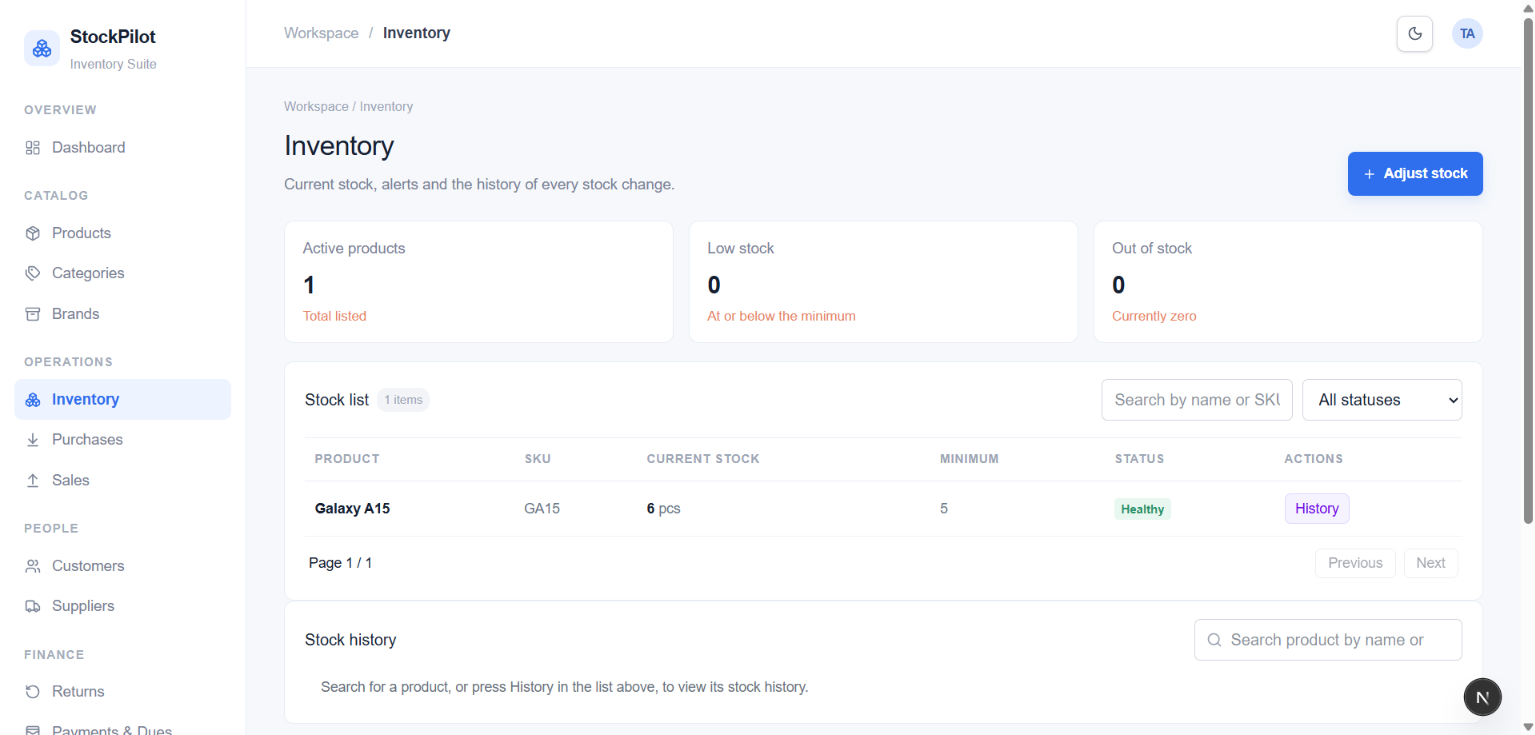
\includegraphics[width=0.97\textwidth]{screenshots/inventory-after-s19.png}}\caption{Inventory after case S19: the stock of the product is 6}\end{figure}
\begin{figure}[H]\centering\fbox{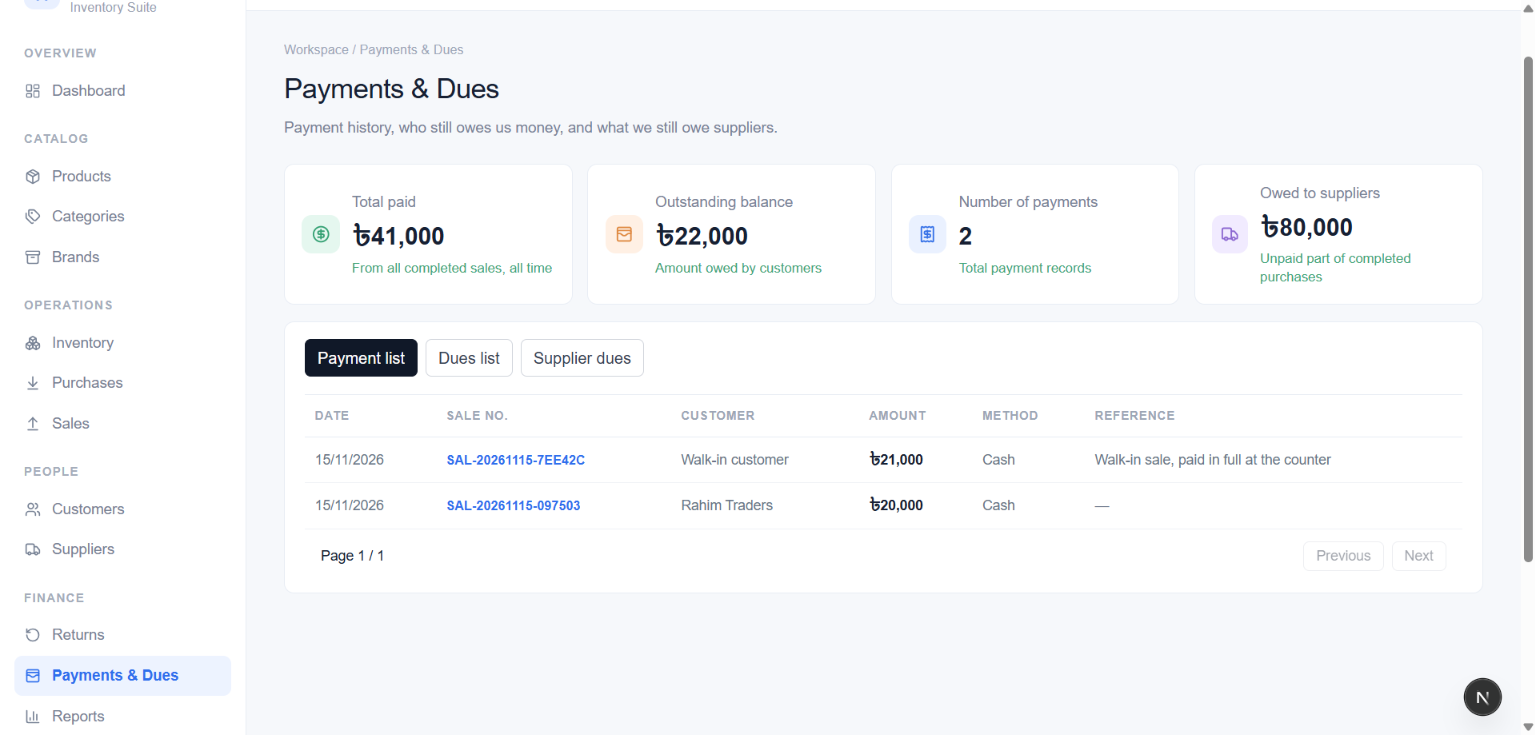
\includegraphics[width=0.97\textwidth]{screenshots/payments-s21.png}}\caption{Case S21: total paid Tk 41,000, customer dues Tk 22,000, owed to suppliers Tk 80,000}\end{figure}
\begin{figure}[H]\centering\fbox{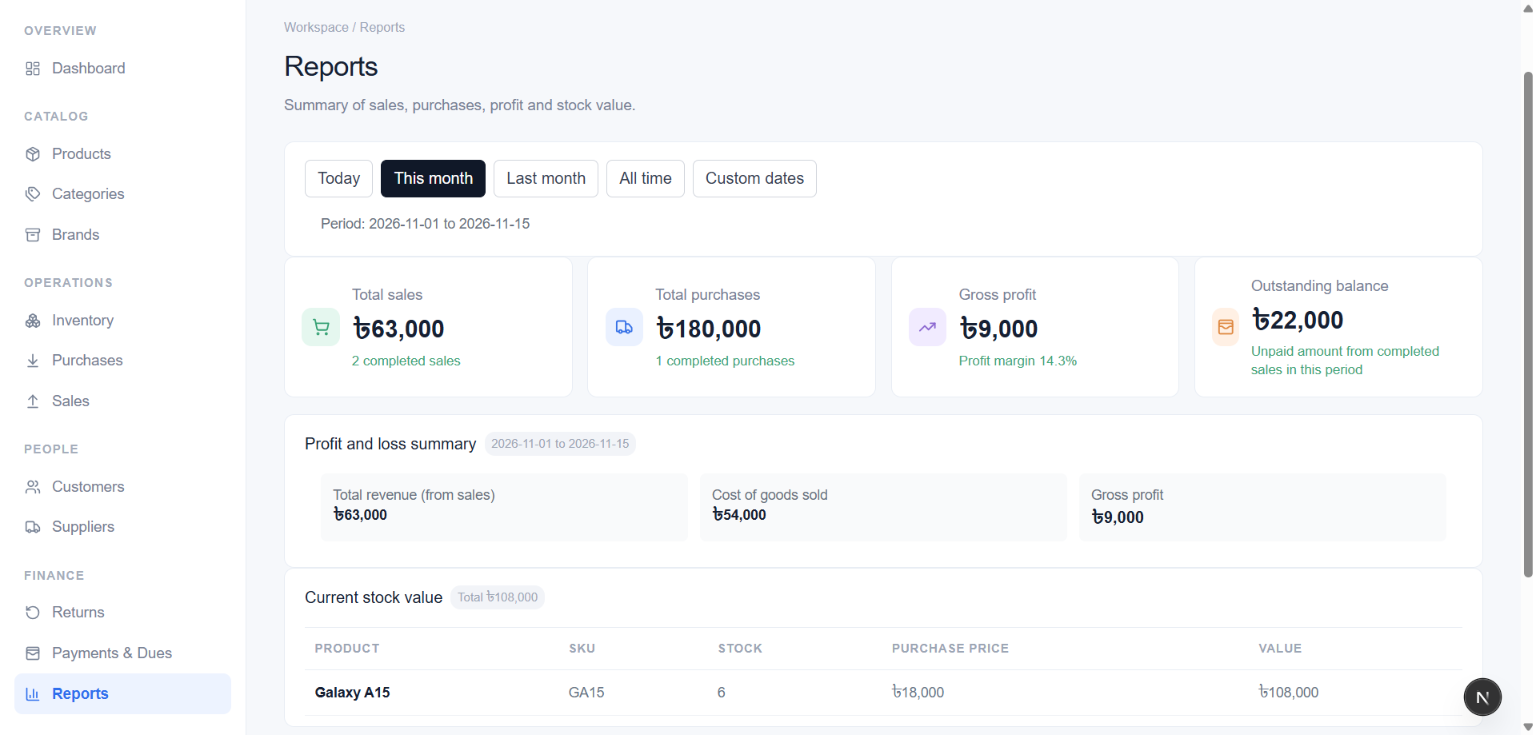
\includegraphics[width=0.97\textwidth]{screenshots/reports-s22.png}}\caption{Case S22: sales Tk 63,000, purchases Tk 180,000, gross profit Tk 9,000, stock value Tk 108,000}\end{figure}

\section{Deployment Tests}
These cases use the live website. They only read data.
\begin{longtable}{@{}P{0.75cm}P{6.0cm}P{5.3cm}P{1.3cm}@{}}
\toprule
\textbf{ID} & \textbf{Steps} & \textbf{Expected result} & \textbf{Result} \\
\midrule
\endhead
L01 & \textbf{Login on the live website.} Open the Vercel address and log in with a real account. & The Dashboard opens with the real figures. The first load can take longer because the free server sleeps. & Not run \\\addlinespace
L02 & \textbf{Search on the live website.} Open Products and search for \code{galaxy}. & Matching products are listed within a few seconds. & Not run \\\addlinespace
L03 & \textbf{The three parts are on three servers.} Open DevTools, Network tab, and reload the Products page. Select the products request. & The page address is on \code{vercel.app}. The Request URL is on \code{onrender.com}. The data comes from MongoDB Atlas. & Not run \\*
\bottomrule
\end{longtable}

\section{Known Limitations}
\begin{itemize}
  \item A return that included a cash refund cannot be cancelled. A new sale is recorded instead.
  \item When a supplier has been paid in full and products are returned afterwards, the money that the supplier owes back is not tracked.
  \item The free backend server sleeps when it is not used, so the first request after a pause is slow.
  \item The system tests are done by hand. Automatic browser tests can be added later.
\end{itemize}

\section{Conclusion}
The database, the backend and the frontend work together as one system. All automatic tests passed: 19 of 19 unit tests, 8 of 8 integration tests and 217 of 217 API checks. Of the 27 system test cases, 21 were run and all of them passed. They cover the whole path of a product (purchase, sale, payment, stock adjustment, return) and the totals on the report pages. 6 system cases (roles in the browser, session, server failure, audit log) and the 3 deployment cases have not been run yet and are marked \emph{Not run}. The role checks and the error handling behind these cases are already covered by the API tests of Step 3.

\end{document}
